\section{Crowdsourcing}
While in the previous sections, we discussed collective intelligence's theoretical origins as an information processing theory and then to analyze the intelligence of small groups. However, Collective Intelligence has become a popular theory to analyze the performance of large groups, such as in MOOCs or in crowdsourcing tasks. 

Generally, crowdsourcing has became popular because many tasks are still too difficult for algorithms, but are too large for a single expert to do. Therefore, the tasks have to be split and organized so people of various skill levels can complete difficult tasks with minimal interaction. We discuss three types of crowdsourcing tasks that the theory could be applied to: directed crowdsourcing, collaborative crowdsourcing, and passive crowdsourcing \cite{crowdsourcing}.

\subsection{Directed Crowdsourcing}
Directed crowdsourcing is what is traditionally thought of when people think of crowdsourcing. Basically, someone thinks of a task, and then they provide some incentive for workers to perform the task. Amazon Mechanical Turk is a popular platform for this type of crowdsourcing, where someone puts up jobs that people take in order to get paid small amounts of money, based on their task completion. 

These types of tasks are both very useful for research but also an interesting subject of research themselves. The tasks often involve things that assist studies, such as labeling data sets for machine learning, or even participating in experiments that scientists have designed to be performed on the platform. Generally, the incentive to do so is money: the workers are compensated financially for performing the tasks by the organizer. However, other methods of compensation would still be considered directed crowdsourcing, so long as the organizer is solely responsible for designing the job and gathering the workers.

In directed crowdsourcing, the interesting problem is to get quality work. Since the tasks generally only employ someone for a single round, and because the number of workers and tasks are so high, there is very little managerial support or supervision to the workers. In other words, if they do not understand the task or the task is too difficult, they may have little motivation to do the task well enough for it to be useful. Generally, even paying more is not very helpful: it will increase the number of people willing to do the task, but it won't increase the average quality of the work \cite{crowdsourcing}. No matter how much the organizer pays, there is little external incentive for the workers to do their absolute best work, because there are few drawbacks to doing mediocre work.

In order to get quality work, the organizers must develop a workflow that minimizes the difficulty of any individual task, and then combines them to get quality work out of it. For instance, the Find-Fix-Verify paradigm has been used for editing documents \cite{crowdsourcing}. The idea of this paradigm is that one worker finds areas where the document doesn't read as well it should, and marks them for the next worker. The next worker then makes corrections to the problem areas that the first worker highlighted. Finally, the last participant looks over the changes that were made to the document and verifies that they were correct. Each of these tasks individually are fairly simple, but they have been shown to give pretty good results \cite{crowdsourcing}. 

Another paradigm for effective work is inspired by distributed computing: Map Reduce. Map and reduce originally refer to two functions in the functional programming paradigm. Map essentially applies some function to each of the elements of a list. Reduce takes elements from a list and combines them into a single structure. This has been popular in distributed computing, because the map on each element can be computed by a computer, and then the reduce can be computed by another computer. Similarly, this type of idea can be performed by humans, where each person, instead of viewing the whole data set, just takes something simple and applies some change to it. Then, the last person combines these outputs into a single output that goes back to the organizer. See Figure \ref{fig:mapreduce}.

\begin{figure}[!h]
\centering
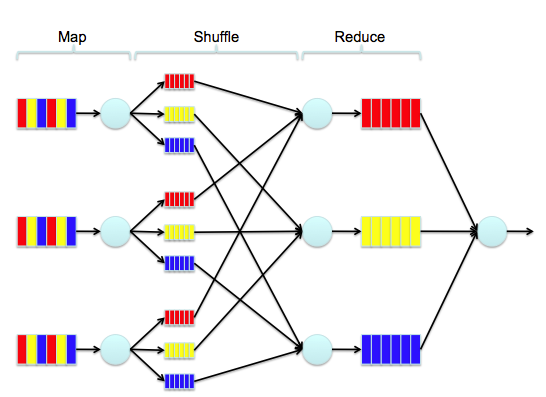
\includegraphics[width=0.9\columnwidth]{figure/mapreduce}
\caption{A visualization of the map reduce workflow}
\label{fig:mapreduce}
\end{figure} 

These types of workflows allow for a complicated task to be broken into many simple tasks. These methods seem to be more effective for getting quality work than increasing pay in the setting of crowdsourcing \cite{crowdsourcing}.

\subsection{Collaborative Crowdsourcing}
Collaborative crowdsourcing does not rely on a single organizer to direct the work. While there is often a person in charge, he or she plays a much more limited role than in directed crowdsourcing. For instance, while Jimmy Wales provides the hosting for Wikipedia, he does not instruct any individual editors on proper editing methodology or topics.

Besides leadership, the primary difference between collaborative crowdsourcing and directed crowdsourcing is the motivation to participate. Generally, people participate in directed crowdsourcing for money; in collaborative crowdsourcing, people participate because they want to. 

This can be for a variety of reasons. For something like Wikipedia, people probably generally participate because they agree in Wikipedia's general mission statement: to disseminate the world's knowledge for free. Those who participate in Stack Overflow (or various open source projects) may do so in part because it helps them build their resume, but many do it because they enjoy it. Likewise, there have been recent efforts in biological sciences to gather people to assist with tasks such as taking pictures when they identify birds \cite{crowdsourcing}. Many people may enjoy the title and the idea of being an amateur scientist and so are willing to help with these types of activities.

Also along this way of reasoning is FoldIt, which has been so successful in recruiting helpers that it appeared in Nature \cite{foldit}. Generally, people participate in FoldIt not just to help scientific advancement, but also because it's fun. FoldIt was designed as a game that happens to model protein arrangements. By playing the game, players are essentially trying to solve puzzles that represent scientific problems, and when they successfully solve the puzzle, scientific discovery is made.

These types of tasks motivate people in various ways, completely depending on the person; what makes it collaborative crowdsourcing is that everyone participates solely because they want to.

\subsection{Passive Crowdsourcing}
In directed crowdsourcing, there are clear participants and a clear organizer. In collaborative crowdsourcing, there's clear participants, but not necessarily a clear organizer. In passive crowdsourcing, there are neither. Passive crowdsourcing can be thought of as using the data that is naturally generated by people as they go about their daily lives. 

For a simple example, museums setup paintings. If they want to know what paintings are the most popular, they can look at how worn the floor tiles are in front of those paintings \cite{crowdsourcing}. For another example, a search engine, instead of having an internal ranking algorithm such as Google's, could rank pages entirely based on how likely it is for user's to click that page after searching for those keywords \cite{crowdsourcing}. This clearly falls into the paradigm of crowdsourcing: users are performing the simple tasks of ranking which web pages are most relevant to their query. However, they do it without even realizing.

Perhaps the most famous example of this is the reCAPTCHA system \cite{recaptcha}. Most people are used to the idea of CAPTCHA, an acronym for Completely Automated Public Turing test to tell Computers and Humans Apart. The idea is that websites can introduce a CAPTCHA that can block automated scripts from accessing it, without blocking humans. This is done by providing a task that humans can fairly easily solve, but is difficult for state of the art algorithms. The most common task at this point is recognizing characters from poorly photocopied books or street signs.

However, reCAPTCHA took this an introduced another element. When using reCAPTCHA, the system itself only has an answer for one of the pieces of text that it has. People enter answers for both pieces of text, however. Then, the system is able to build a consensus on what the second piece of text says. 

Again, this is very reminiscent of crowdsourcing: it's easy to imagine the exact same task on Mechanical Turk. What makes it passive crowdsourcing is that the participants do not even necessarily know they are participating.